%\documentclass[12pt,twoside]{article}
%\usepackage[inner=1in,outer=0.6in,top=0.7in,bottom=1in]{geometry}
%\usepackage{fontspec}
%\usepackage{xeCJK}
%\setmainfont{Times New Roman}
%\setsansfont{Verdana}
%\setmonofont{Courier New}                    % tt
%\setCJKmainfont{微軟正黑體}
%\setCJKfamilyfont{kai}{標楷體}		% for changing the title font in title.pgf -> have to manually 
%\usepackage{graphicx}
%\usepackage{pgf}
%\usepackage{pstricks,pst-node}
%
%\renewcommand{\today}{西元\number \year 年\ifcase \month \or 1月\or 2月\or 3月\or 4月\or 5月\or 6月\or 7月\or 8月\or 9月\or 10月\or 11月\or 12月\fi
%} 
%
%\begin{document}

\begin{pspicture}(6in,2in)
%\psgrid

\rput[B](13 cm,-1.25cm){
\rnode{A}{
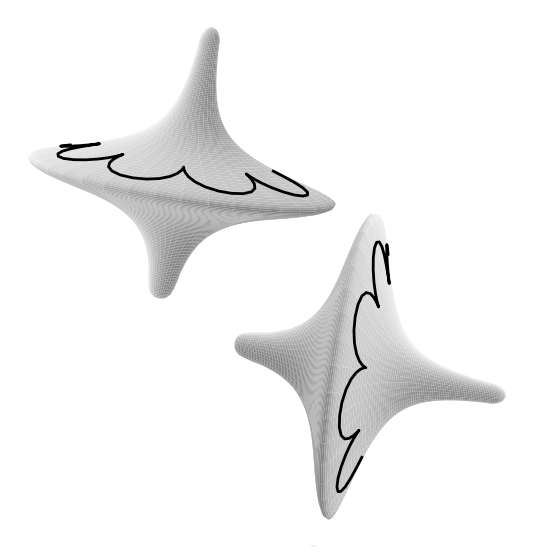
\includegraphics[scale=0.37]{./otherstuff/logo_Aug29_test.PNG}%../
}}

\rput[bl](-0.1cm,-0.2cm){
\rnode{B}{

\includegraphics[scale=0.6]{./otherstuff/gyro_title_line4.PNG}%./otherstuff/
}}
\psline(0.2cm,-0.3cm)(11.3cm,-0.3cm)
\psline(0.2cm,2.0cm)(12.3cm,2.0cm)



\rput[tl](0.2cm,5.4cm){
\rnode{C}{
\large \textcolor{gray}{
\parbox{13cm}{從基礎的貼體角速度與牛頓尤拉方程簡單地衍伸到\\姿態估測法與積分器,並且模擬陀螺3D章動進動。}
}
}}

\rput[bl](2cm,2.5cm){
\rnode{D}{
\large 小良,台南,\today
}}

\rput[B](5.5 cm,3.3cm){
\rnode{E}{
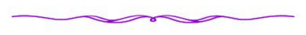
\includegraphics[scale=0.5]{./otherstuff/decoration_line.PNG}%../
}}





\end{pspicture}


%\end{document}